\subsection*{Teil A: Achsenspiegelung verstehen (25 Minuten)}

\begin{enumerate}[label=\arabic*.]
    \item \textbf{Spiegle die Punkte an der senkrechten Achse:}
    \textit{Tipp: Miss den Abstand zur Achse und trage ihn auf der anderen Seite ab}
    \vspace{0.5cm}

    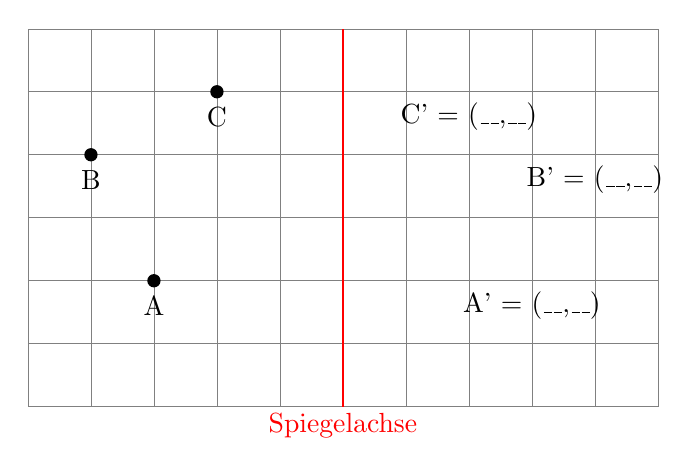
\begin{tikzpicture}[scale=0.8]
        \draw[step=1cm,gray,very thin] (0,0) grid (10,6);
        \draw[thick,red] (5,0) -- (5,6);
        \node[red] at (5,-0.3) {Spiegelachse};
        \fill (2,2) circle (3pt);
        \node at (2,1.6) {A};
        \fill (1,4) circle (3pt);
        \node at (1,3.6) {B};
        \fill (3,5) circle (3pt);
        \node at (3,4.6) {C};
        \node at (8,1.6) {A' = (\_\_,\_\_)};
        \node at (9,3.6) {B' = (\_\_,\_\_)};
        \node at (7,4.6) {C' = (\_\_,\_\_)};
    \end{tikzpicture}

    \vspace{1cm}

    \item \textbf{Zeichne die Spiegelachse zwischen P und P':}
    \textit{Tipp: Die Spiegelachse steht senkrecht auf der Verbindungslinie und geht durch die Mitte}
    \vspace{0.5cm}

    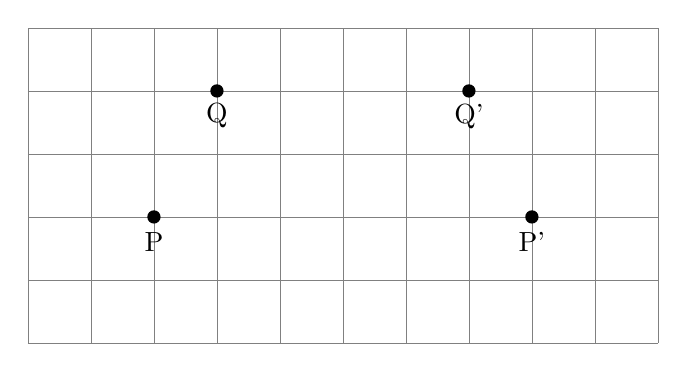
\begin{tikzpicture}[scale=0.8]
        \draw[step=1cm,gray,very thin] (0,0) grid (10,5);
        \fill (2,2) circle (3pt);
        \node at (2,1.6) {P};
        \fill (8,2) circle (3pt);
        \node at (8,1.6) {P'};
        \fill (3,4) circle (3pt);
        \node at (3,3.6) {Q};
        \fill (7,4) circle (3pt);
        \node at (7,3.6) {Q'};
    \end{tikzpicture}

    \vspace{1cm}

    \item \textbf{Vervollständige die gespiegelten Figuren:}
    \vspace{0.5cm}

    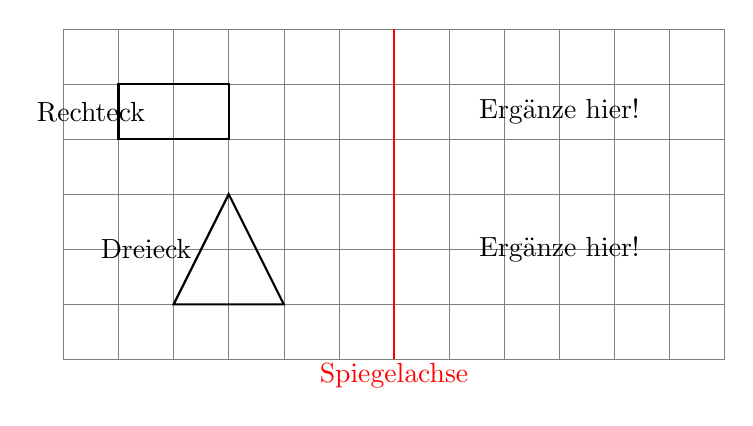
\begin{tikzpicture}[scale=0.7]
        \draw[step=1cm,gray,very thin] (0,0) grid (12,6);
        \draw[thick,red] (6,0) -- (6,6);
        \node[red] at (6,-0.3) {Spiegelachse};
        % Dreieck links
        \draw[thick] (2,1) -- (4,1) -- (3,3) -- cycle;
        \node at (1.5,2) {Dreieck};
        % Rechteck links (halb)
        \draw[thick] (1,4) -- (3,4) -- (3,5) -- (1,5) -- cycle;
        \node at (0.5,4.5) {Rechteck};
        % Schüler sollen rechts ergänzen
        \node at (9,2) {Ergänze hier!};
        \node at (9,4.5) {Ergänze hier!};
    \end{tikzpicture}
\end{enumerate}